% !TEX encoding = UTF-8 Unicode 
\setchapterstyle{kao}
\setchapterpreamble[u]{\margintoc}
\chapter{UNITÉS ET DIMENSIONS}
\labch{unites_et_dimensions}


\blockquote[Bachelard]{Dis-moi comment l'on te cherche, je te dirai qui tu es}

\begin{center}
\textbf{Version en ligne}

\url{https://femto-physique.fr/omp/grandeurs-physiques.php}
\end{center}

\section[Dimension d'une grandeur]{Dimension d'une grandeurs physique}
\subsection{Grandeurs physiques}
Une grandeur physique est une quantité qui se rapporte à une propriété  et qui peut se mesurer. Or, \textbf{mesurer, c'est comparer}. C'est comparer à l'aide d'un instrument, une grandeur physique inconnue avec une grandeur de même nature -- on dira\textbf{ de même dimension} -- prise comme référence que l'on appelle \textbf{étalon}. 

Par exemple, le poids de Miss Univers peut être comparé à celui d'un étalon (1 kg par exemple) à l'aide d'une balance : le poids de Miss Univers est une grandeur physique. En revanche, sa beauté est une propriété subjective qui ne peut être mesurée compte tenu qu'il n'existe pas d'étalon de beauté. En d'autres termes, la beauté se rapporte à l'aspect physique mais ne relève pas de la Physique ; il ne s'agit pas d'une grandeur physique.

Lors du processus de mesure (mesurage) on effectue donc une comparaison entre un étalon (l'unité) et la grandeur à mesurer puis  l'on traduit le résultat par un chiffre (la mesure) assortie d'un intervalle définissant un certain niveau de confiance (l'incertitude) ainsi que l'unité\sidenote[][]{L'unité est indispensable ! Exprimer le résultat d'un calcul ou d'une mesure sans préciser l'unité n'a aucun sens.}
\[
X=x_\text{m}\pm\Delta x\quad\text{unité}
\] 
La détermination de la mesure et de l'incertitude fait l'objet d'un autre chapitre. Ici on s'intéresse au contenu dimensionnel des grandeurs physiques et du choix de l'unité.

\subsection{Notion de dimension}
En général, le résultat d'une mesure dépend de l'étalon utilisé. Par exemple, si l'on compare la longueur $\ell$ d'une règle de 1~m avec un décimètre, on obtient $\ell=10$~dm. Si l'on choisit un double décimètre comme étalon de mesure, on trouve $\ell=5$~ddm (double décimètre). La mesure est donc différente ($5\neq 10$) : on dit que  la longueur possède une dimension.
\newpage
\begin{kaobox}[frametitle=Dimension d'une grandeur]
Par définition, une grandeur physique $G$ a une dimension si sa mesure dépend du choix de l'étalon de mesure. Sa dimension est notée $[G]$.
\end{kaobox}
Il ne faut pas confondre cette notion avec l'unité qui est purement conventionnelle alors que la dimension est une propriété indépendante de tout système d'unités.

Deux grandeurs ont même dimension si on peut les comparer. C'est pourquoi le rayon d'un cercle et son périmètre ont même dimension, car je peux en faire la mesure avec le même étalon (par exemple un fil souple d'une certaine longueur). Ici il s'agit de la dimension [longueur].

Il existe également des grandeurs physiques sans dimension (on dit aussi adimensionnées). Dans ce cas la dimension est noté $[G]=1$. Par exemple, l'angle $\theta$ d'un secteur AOB est une grandeur que l'on peut mesurer comme suit : traçons un cercle de centre O et de rayon  $r$. Les droites (OA) et (OB) coupent le cercle en deux points A' et B'. L'angle se mesure en faisant le rapport de la longueur d'arc $\arcdecercle{A'B'}$ et du rayon du cercle.
\begin{marginfigure}
\centering
	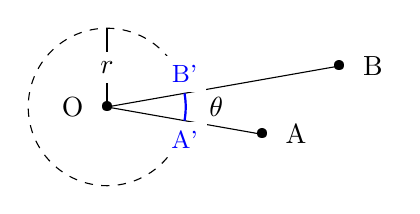
\begin{tikzpicture}
	\draw (10:3)node{•}node[right=5pt]{B}--(0,0)node{•}node[left=5pt]{O}--(-10:2)node{•}node[right=5pt]{A};
	\draw[dashed] (0,0) circle(1);
	\draw[thick,blue] (-10:1)node[below,fill=white]{\small A'} arc(-10:10:1)node[above,fill=white]{\small B'};
	\draw (0,0)--(90:1)node[midway,fill=white]{$r$};
	\draw (0:1)node[right=5pt]{$\theta$};
	\end{tikzpicture}
\caption{Définition de l'angle plan.}
\labfig{définition_de_l_angle_plan}
\end{marginfigure}
\[
	\theta\stackrel{\text{def}}= \dfrac{\arcdecercle{A'B'}}{r}
\]
\begin{margintable}
\centering
\footnotesize
\caption{Symbole donné aux dimensions des grandeurs de base.}
\labtab{lettre_donnee_aux_dimensions_des_grandeurs_de_base}
	\begin{tabular}{lc}
		\toprule
		\textbf{Dimension}		& \textbf{Symbole}	\\
		Longueur				& L			\\
		Masse					& M			\\
		Temps					& T			\\
		Intensité électrique	& I			\\
		Température				& $\Theta$	\\	
		Quantité de matière		& N\\
		\bottomrule
	\end{tabular}
\end{margintable}
On constate donc que si l'on double le rayon du cercle, la longueur d'arc double également de sorte que l'angle ne dépend pas de la taille du cercle. Il est alors assez évident que si l'on décide de mesurer les distances en centimètre, en pouce, ou dans n'importe quel système d'unités, le résultat de l'angle $\theta$ ne changera pas. \textbf{L'angle est donc sans dimension}. De la même manière, une grandeur définie comme le rapport de deux grandeurs de même dimension, ne présente pas de dimension. 

Enfin, par commodité, on a donné un nom spécifique à  certaines dimensions (cf. \reftab{lettre_donnee_aux_dimensions_des_grandeurs_de_base}).



\subsection{Équation aux dimensions}	
Une loi physique affirme l'égalité de deux grandeurs qui sont nécessairement de même nature. Une loi physique est donc aussi une relation entre différentes dimensions : on parle d'\textbf{équation aux dimensions}. 
Voyons comment obtenir ces équations aux dimensions sur quelques exemples. 
\begin{description}
	\item[La vitesse :] d'après la définition $v_x\stackrel{\text{def}}=\mathrm{d}x/\mathrm{d}t$, on déduit 
	\[[v]=\mathrm{LT^{-1}}\]
	\item[L'accélération :] la définition $a_x\stackrel{\text{def}}=\mathrm{d}v_x/\mathrm{d}t$ donne 
	\[[a]=\frac{[v]}{\text{T}}=\mathrm{LT^{-2}}\]
	\item[La force :] en vertu de la deuxième loi de Newton $F=ma$ on a 
	\[[\text{F}]=\mathrm{MLT^{-2}}\] 
	\item[La constante des gaz parfaits :] on peut obtenir sa dimension à partir de la loi du gaz parfait $pV=nRT$.  
	\[ [R]=\frac{[p][V]}{[n][T]}=\frac{[F]}{\mathrm{L^{2}}}\times\frac{\mathrm{L^3}}{N\Theta}=
	\mathrm{ML^2}\mathrm{T^{-2}}\Theta^{-1}\mathrm{N^{-1}}\]	
	\item[Le champ magnétique :] par définition du champ magnétique, une particule de charge électrique 
	$q$ se déplaçant à la vitesse $\overrightarrow{v}$ dans un champ magnétique $\overrightarrow{B}$ subit une force 
	$\overrightarrow{F}=q\overrightarrow{v}\wedge\overrightarrow{B}$, d'où
	\[ [B]=\frac{[F]}{[q][v]}=\frac{\mathrm{MLT}^{-2}}{\mathrm{IT}\times \mathrm{LT}^{-1}}=\mathrm{MT}^{-2}\mathrm{I}^{-1}\]
\end{description}



\section[Le SI]{Le Système international d'unités}
Comme on l'a déjà dit, mesurer c'est comparer une grandeur physique avec un étalon qui définit l'\textbf{unité de mesure}. Celle-ci relevant d'un choix arbitraire il faut bien  \textbf{convenir} d'un système d'unités pour pouvoir communiquer (transactions commerciales, rapports scientifiques, etc.). La bonne idée consiste alors à choisir des étalons dont la définition est indépendante du lieu et du temps et avec lesquels on peut construire toutes les unités. C'est l'ambition du Système international d'unités (SI) adopté par quasiment tous les pays\sidenote{Trois pays n'ont pas encore adopté officiellement le système métrique : le Libéria, la Birmanie et… les Etats-Unis.}. Né officiellement en 1960, il s'agit d'une extension de l'ancien système MKSA. 

 
\subsection{Les unités de base} 
\begin{marginfigure}[*6]
\centering
	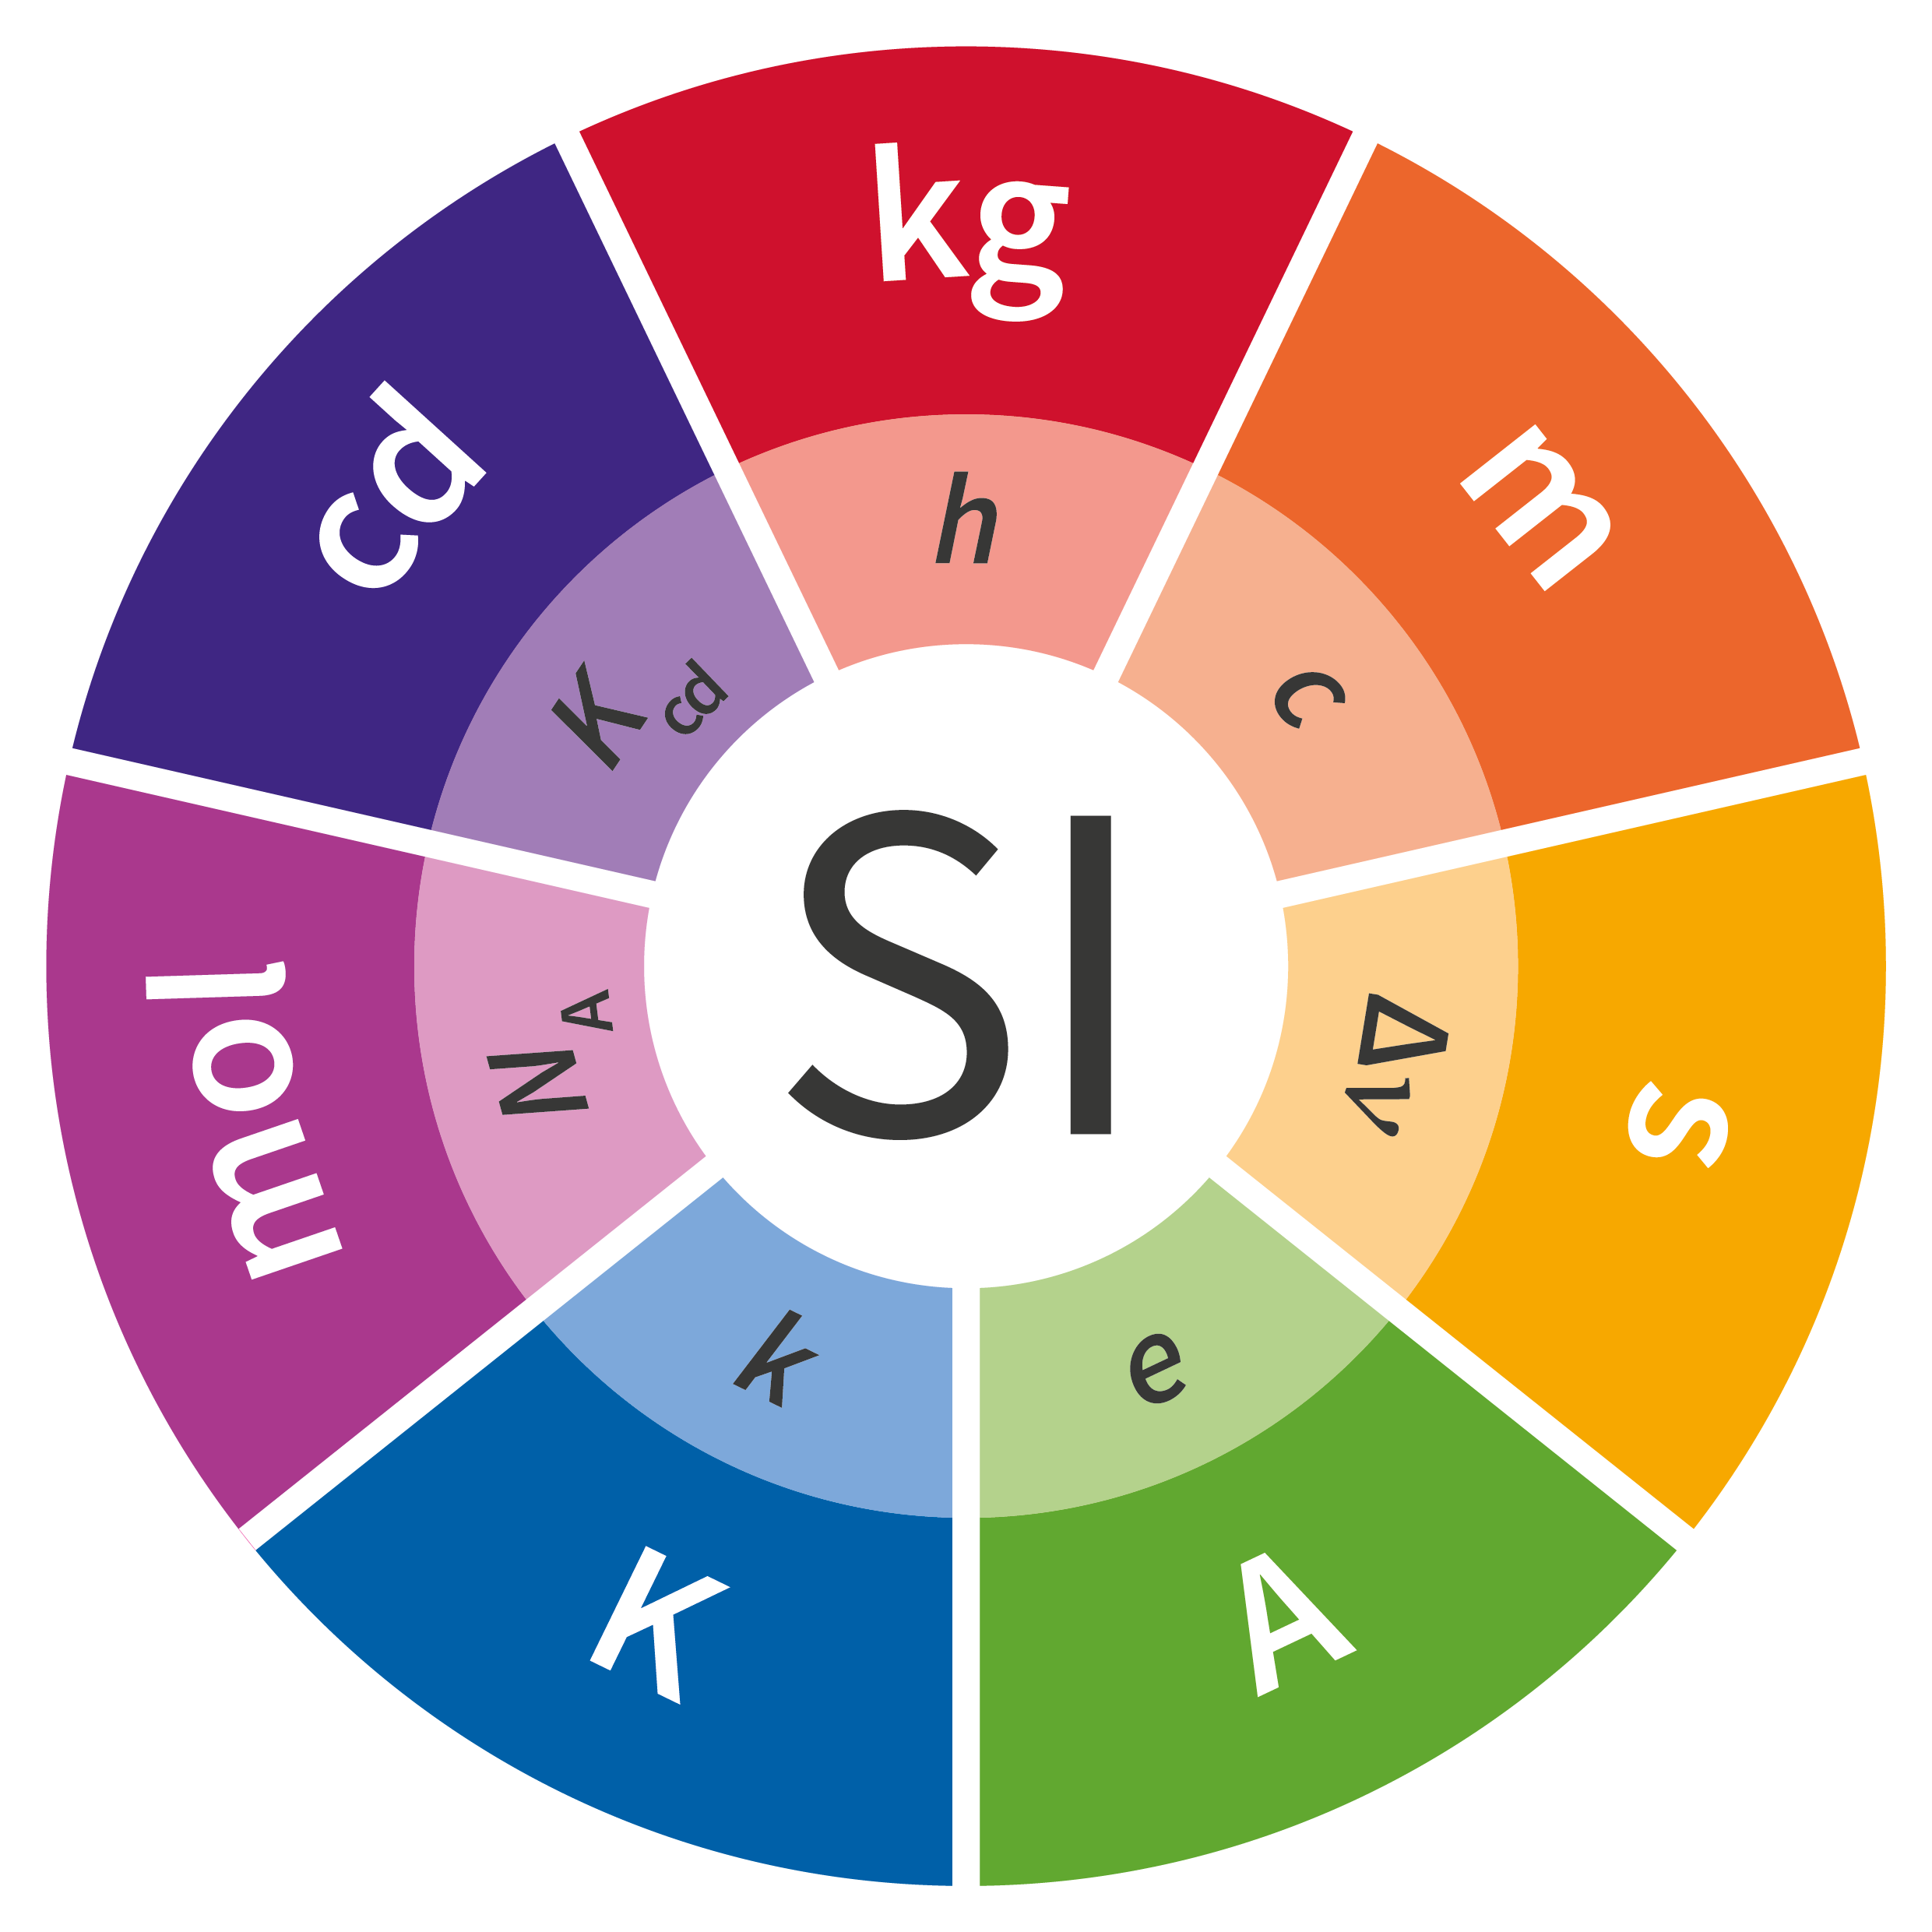
\includegraphics[width=5cm]{img/SI-Illustration-Constants-Colour-Full.png}
\caption{Le SI et ses 7 unités fondamentales liées aux 7 constantes universelles.}
\labfig{title_name}
\end{marginfigure}
Le (SI) forme un système cohérent reposant sur \textbf{sept unités de base} (\emph{cf.} \reftab{sept_unites_de_base}) indépendants du point de vue dimensionnel. 
\begin{table}[ht!]
	\centering
	\footnotesize
	\caption{Les sept unités de base du Système internationale d'unités.}
	\labtab{sept_unites_de_base}	
	\begin{tabular}{lcrr}
		\toprule
		\textbf{Dimension}		& \textbf{Symbole}	& \textbf{Unité SI}	&\textbf{Symbole}\\
		Longueur							& L									& mètre						& m\\
		Masse									& M									& kilogramme			& kg\\
		Temps									& T									& seconde					& s\\
		Intensité électrique	& I									& ampère					& A\\
		Température						& $\Theta$					& kelvin					& K\\
		Quantité de matière		& N									& mole						& mol\\
		Intensité lumineuse		& J									& candela					&cd\\
		\bottomrule
		\end{tabular}
\end{table}
Depuis le 20 mai 2019, les unités du SI sont définies à partir de sept constantes de la nature auxquelles on donne une valeur fixe. Les sept constantes sur lesquelles repose le Système international d'unités sont
\begin{itemize}
\item la fréquence de la transition hyperfine du césium 133 \(\Delta \nu_\textsf{Cs}=9\,192\,631\,770\,\mathrm{Hz}\) qui permet de définir la seconde ;
\item la vitesse de la lumière dans le vide \(c=299~792~458\,\mathrm{m.s^{-1}}\) qui permet de relier le mètre à la seconde ;
\item la constante de Planck \(h=6{,}626~070~15\cdot 10^{-34}\,\mathrm{kg.m^2.s^{-1}}\) qui définit indirectement le kilogramme ;
\item la charge élémentaire \(e=1{,}602~176~634\cdot 10^{-19}\,\mathrm{C}\) qui fixe l'ampère puisque \(1\,\mathrm{C}=1\,\mathrm{A.s}\) ;
\item la constante de Boltzmann \(k_\text{B}=1{,}380~649 \cdot 10^{-23} \, \mathrm{J.K^{-1} } \) qui relie le kelvin aux unités mécaniques ;
\item la constante d'Avogadro \(N_\text{A}=6{,}022~140~76\cdot 10^{23}\,\mathrm{mol^{-1}}\) qui donne le nombre exact d'entités élémentaires (atomes, molécules, ions, etc.) formant une mole ;
\item Enfin, l'efficacité lumineuse \(K_{cd}=683\,\mathrm{lumen.W^{-1}}\) pour un rayonnement monochromatique de longueur d'onde\sidenote[][]{Cette longueur d'onde correspond au maximum de sensibilité de l'œil humain.} \(\lambda=555\,\mathrm{nm}\). Cette constante relie les grandeurs sensorielles (intensité en candela, éclairement en lux, flux lumineux en lumen) aux grandeurs énergétiques de la lumière (intensité en watt par stéradian, éclairement en watt par mètre carré, flux en watt).
\end{itemize}
Notez que ces constantes sont des grandeurs physiques sans incertitude. En revanche, certaines grandeurs auparavant fixées (avant mai 2019) retrouvent leur statut de grandeur expérimentale. Par exemple, une mole de carbone 12 pesait auparavant 12~g par définition ; dorénavant sa valeur n'est plus connue exactement. Elle présente donc une incertitude.



%\begin{description}
%	\item[Le mètre] est relié à la seconde \emph{via} l'invariance de la vitesse de la lumière dans le vide. Par définition, la distance parcourue par la lumière dans le vide pendant une seconde vaut $L=299\,792\,458\, \rm m$
%
%\remarque{le mètre a connu en deux siècles quatre définitions successives. Initialement, le mètre était défini à partir de la longueur du méridien terrestre supposé invariable: $L=40\,000\;{\rm km}$. Aujourd'hui, avec l'étalon mètre actuel (lié à l'étalon seconde) $L=40\,008,08\;{\rm km}$ ; la différence est donc imperceptible pour un utilisateur courant.}
%	
%	\item[Le kilogramme] est la masse d'un bloc cylindrique de Platine irridié (90\%Pt-10\%Ir) conservé au pavillon de Breteuil (Sèvres) depuis 1889. 
%	
%	\remarque{cet étalon se dégrade par usure et contamination ; c'est pourquoi il est envisagé de changer de définition du kg et de définir cette unité à partir de la constante de Planck $h$.}
%
%	\item[La seconde] est la durée de $9\,192\,631\,770$ périodes de la radiation correspondante à la transition entre les deux niveaux hyperfins de l'état fondamental de l'atome $\mathrm{_{133}Cs}$ au repos dans le référentiel d'étude.
%	
%	\remarque{initialement la seconde était définie à partir du jour solaire moyen J par la relation $J=86400\,{\rm s}$. Aujourd'hui, avec la définition de l'étalon seconde, on a $J=86400,003\,{\rm s}$.}
%
%	\item[L'ampère] est défini à partir de la force magnétique de Laplace et permet d'établir à $10^{-7}$ près les principaux étalons du domaine électrique. Un ampère est l'intensité du courant qui fait apparaître une force de $2.10^{-7}\;\mathrm{N}$ entre deux conducteurs filiformes rectilignes infinis distants de $1\;\mathrm{m}$, parcourus par ce courant électrique.
%	
%	\remarque{cette définition fixe les valeurs de la perméabilité magnétique et de la permittivité du vide à
%			\[\mu_{0}=4\pi.10^{-7}\;\mathrm{H.m^{-1}}\quad\text{et}\quad\epsilon_0=\frac{1}{\mu_0 c^2}\]
%	Notez qu'il est prévu de redéfinir l'ampère à partir de la charge de l'électron $e$ ce qui aura pour effet de fixer la valeur de $e$ mais de rendre à $\mu_0$ et à $\epsilon_0$ leur statut de constantes expérimentales.}
%	
%	\item[Le kelvin] se rapporte à la loi du gaz parfait. Par définition du kelvin, la température d'un gaz parfait en équilibre avec l'eau dans ses trois états (le point triple de l'eau) vaut $273,16\;\mathrm{K}$.
%	
%	\remarque{la future définition du kelvin fixera la valeur de la constante de Boltzmann $k_{\rm B}$.}
%	
%	\item[La mole] est la quantité d'atomes contenue dans 12~g de carbone 12. 
%	
%	\remarque{l'imprécision de cet étalon est donc liée à celle de la masse. Pour pallier cet inconvénient, il est envisagé de définir la mole en fixant la valeur du nombre d'Avogadro.}
%
%	\item[La candela] est l'unité donnant l'intensité lumineuse d'une source dans une direction donnée. Par définition, 1~cd est intensité lumineuse d'une lumière verte de fréquence $\nu=540.10^{12}\;\mathrm{Hz}$ rayonnant $\dfrac{1}{683}\;\mathrm{W.sr^{-1}}$.
%\end{description}


\subsection{Les unités dérivées}
Les sept unités de base du système international sont les «unités fondamentales» à partir desquelles sont obtenues par combinaison toutes les autres unités, dites \textbf{unités dérivées}. Certaines d'entre-elles se sont vues attribuer un nom qui rappelle une personnalité scientifique: newton, pascal, joule, volt, tesla, henry etc.
\begin{table}[htbp]
	\caption{Quelques unités dérivées.}
	\labtab{unites-derivees}
	\footnotesize
	\begin{tabular}{lrlr}
	\toprule
	\textbf{Grandeur}					&\textbf{Unité SI}
	&
	\textbf{Grandeur}					&\textbf{Unité SI} \\
	\midrule
	aire								& $\mathrm{m^{2}}$ 
	&énergies 							& J	(joule)\\	

	volume								& $\mathrm{m^{3}}$  
	&pression							& Pa (pascal)\\

	masse molaire						& $\mathrm{kg.mol^{-1}}$ 
	&tension								& V (volt)\\

	masse volumique 					& $\mathrm{kg.m^{-3}}$ 
	&charge électrique					& C (coulomb)\\

	fréquence							& Hz (hertz)
	&résistance électrique				& $\Omega$ (ohm)\\

	vitesse (scalaire)					& $\mathrm{m.s^{-1}}$ 
	&champ électrique					& $\mathrm{V.m^{-1}}$\\

	vitesse angulaire, pulsation		& $\mathrm{rad.s^{-1}}$ 
	&conductance électrique				& S (siemens)\\

	accélération (scalaire) 			& $\mathrm{m.s^{-2}}$ 
	&capacité électrique					& F (farad)\\

	force d'interaction 				& N (newton)
	&inductance							& H (henry)\\

	puissance mécanique					& W (watt)	
	&champ magnétique					& T (tesla)\\	   
	\bottomrule
	\end{tabular}
\end{table}
Il peut donc y avoir différentes façons d'exprimer la même unité.	

\begin{kaoexample}[frametitle=Exemple : unités de la pression]
La pression s'exprime en pascal (Pa) dans le système international. Etant donné que la pression représente une force par unité de surface on peut aussi l'exprimer en $\mathrm{N/m^2}$. Par ailleurs, on sait d'après l'équation aux dimensions $\mathrm{F=MLT^{-2}}$, que $1\;\mathrm{N}=1\;\mathrm{kg.m.s^{-2}}$ d'où l'on déduit 
\[
1\;\mathrm{Pa}=1\;\mathrm{N.m^{-2}}=1\;\mathrm{kg.m^{-1}.s^{-2}}
\]
\end{kaoexample} 
 
\begin{kaoremark}
Il existe une dernière classe d'unités qu'on appelle unités supplémentaires. Cette classe contient deux unités sans dimension : le radian (rad), unité de l'angle plan, et le stéradian (sr), unité d'angle solide.
\end{kaoremark} 


\subsection{Préfixes SI}	
Enfin, on utilise parfois des préfixes multiplicateurs pour remplacer les puissances de 10 : 
\begin{table}[h!tbp]
	\caption{Préfixes multiplicateurs.}
	\labtab{prefixe-multiplicateurs}
	\footnotesize
\begin{tabular}{lcccccccc}
\toprule
Valeur &	$10^{-18}$ &	$10^{-15}$ &	$10^{-12}$ &	$10^{-9}$ &	$10^{-6}$ &	$10^{-3}$ &	$10^{-2}$ &	$10^{-1}$ \\
Préfixe &	atto &	femto &	pico &	nano &	micro &	milli &centi & déci \\
Symbole	& a	& f	& p	& n	& $\mu$	& m & c & d	\\
\midrule
\midrule
Valeur &	$10$	& $10^{2}$	& $10^{3}$	& $10^{6}$	& $10^{9}$	& $10^{12}$	& $10^{15}$	& $10^{18}$ \\
Préfixe &	déca	& hecto		& kilo 		& Mega		& Giga 		& Tera 		& Peta 		&	Exa \\
Symbole	& da& h	& k	& M	& G	& T	& P &	E \\
\bottomrule
\end{tabular}
\end{table}

\section{Analyse dimensionnelle}
Analyser le contenu dimensionnel d'une relation permet de rendre bien des services. En voici un petit tour d'horizon ...
\subsection{Vérifier une formule}
Une loi physique impose une contrainte qui n'existe pas en mathématique ; elle doit être \textbf{homogène}, c'est-à-dire constituée de termes de même dimension. Sommer deux grandeurs de dimension différente n'a aucun sens en physique. Ainsi pour vérifier une loi physique, la première chose à faire est de vérifier l'homogénéité !	
\begin{kaobox}[frametitle=Vérifier une formule]
	Toute formule non homogène est nécessairement fausse. On retiendra quelques règles :
\begin{itemize}
	\item dans $\sin x$, $\cos x$, $\mathrm{e}^x$, $\ln x$ et $\log x$ la grandeur $x$ doit être sans dimension ;
	\item dans $1+x$, la grandeur $x$ doit être sans dimension ;
	\item dans $1+x/y$, les grandeurs $x$ et $y$ sont de même dimension.
\end{itemize}
\end{kaobox}


\exercice{La période d'oscillation d'un pendule simple dépend de sa longueur $\ell$, du champ de pesanteur $g$ et de l'amplitude angulaire $\theta_\text{max}$ des oscillations. On propose plusieurs formules ; préciser celles qui ne sont pas homogènes :
\begin{multicols}{2}
	\begin{itemize}[label=$\square$]
		\item $T=2\pi\sqrt{\dfrac{\ell+\theta_\text{max}}{g-\theta_\text{max}}}$
		\item $T=2\pi\sqrt{\dfrac{\ell}{g\theta_\text{max}}}$
		\item $T=2\pi\sqrt{\dfrac{\ell}{g}}\left(1+\dfrac{{\theta_\text{max}}^2}{16}\right)$
		\item $T=2\pi\sqrt{\dfrac{\ell}{g}}\left(1+\dfrac{\theta_\text{max}}{\ell}\right)$
	\end{itemize}
\end{multicols}}

Bien entendu, cela ne signifie pas qu'une formule homogène soit forcément exacte, mais cela permet déjà de trier ce qui n'a aucun sens physique de ce qui peut en avoir. De manière générale, l'analyse dimensionnelle est un outil de réfutation, pas de validation.

\begin{kaoremark}
Il faut prendre garde à certaines formules qui mélangent expressions numériques et littérales. Par exemple, le pH d'une solution acido-basique diluée est souvent défini par 
	\[\text{pH}=-\log\left[\mathsf{H_3O^+}\right]\]
Or la concentration n'est pas sans dimension ce qui suggère que cette formule est non-homogène. En réalité cette formule n'obéit pas à la règle élémentaire qui veut que toute relation soit indépendante du système d'unités. En effet, dans la formule qui donne le pH, il est sous entendu qu'il faut exprimer $\left[\mathsf{H_3O^+}\right]$ en mol.L$^{-1}$. Si l'on veut donner la relation qui donne le pH quel que soit le système d'unités on écrira plutôt
	\[\text{pH}=-\log\frac{\left[\mathsf{H_3O^+}\right]}{c^{\circ}}\]
où $c^{\circ}$ désigne la concentration standard. Dans le SI, $c^{\circ}=1000\;\mathrm{mol.m^{-3}}$ mais si l'on décide d'exprimer les concentrations en mol.L$^{-1}$, on a $c^{\circ}=1\;\mathrm{mol.L^{-1}}$ et dans ce cas la tentation est grande de faire disparaître cette constante par commodité. Mais cela ne doit pas nous faire oublier sa présence.
\end{kaoremark} 



\subsection{Conversion d'unités}
L'équation aux dimensions étant indépendante du système d'unités, elle est très utile quand il faut convertir une unité d'un système vers celle d'un autre système. 

\begin{kaoexample}[frametitle=Exemple : la dyne]
Dans le Système International, la force s'exprime en newton alors qu'elle s'exprime en dyne dans le Système CGS (cm, gramme, seconde). Combien de newton vaut 1 dyne ?

L'équation aux dimensions $[\text{Force}]=\mathrm{MLT^{-2}}$ doit être vérifiée dans tout système d'unités. On a donc
	\[\text{1 newton}=\mathrm{1\, kg.m.s^{-2}}\quad\text{et}\quad \text{1 dyne}=\mathrm{1\, g.cm.s^{-2}}\]
Ainsi on en déduit la conversion : 
	\[1\;\mathrm{newton}=10^5\;\mathrm{dynes}\]
\end{kaoexample} 

\subsection{Modéliser}
L'analyse dimensionnelle permet de prévoir la forme d'une loi si l'on sait quels sont les paramètres pertinents du problème.

Supposons par exemple que nous cherchions à exprimer une grandeur $G$ en fonction de 2 paramètres pertinents indépendants $p_{1}$ et $p_{2}$. La méthode consiste alors à trouver comment multiplier $p_1$ et $p_2$ pour former une grandeur de  même dimension que $G$. On écrit donc 
	\[G=\mathrm{C^{te}}{p_1}^\alpha\,{p_2}^\beta\]
où $\alpha$ et $\beta$ sont des facteurs que l'on détermine grâce à l'équation aux dimensions. Une fois ces constantes déterminées, on peut proposer la forme générale de la loi recherchée.

\begin{kaoexample}[frametitle=Exemple : période d'oscillation $T$ d'un pendule simple]
On suppose que la période $T$ dépend de la masse $m$, du champ de pesanteur $g$ et de la longueur $\ell$ du pendule : $T=f(m,g,\ell)$. On écrit alors 
	\[T=\mathrm{C^{te}}m^{\alpha}\,g^{\beta}\,\ell^{\gamma}\]	
où $\mathrm{C^{te}}$ est un facteur adimensioné. Cela nous donne l'équation aux dimensions 
	\[\mathrm{T}=\mathrm{M}^{\alpha}\mathrm{L}^{\gamma+\beta}\mathrm{T}^{-2\beta}\]
La loi devant être homogène on doit poser $\alpha=0$, $\beta=-1/2$ et $\gamma=1/2$. La forme générale est donc 
	\[T=\mathrm{C^{te}}\sqrt{\frac{\ell}{g}}\]
Attention, ce n'est pas parce que l'on trouve une loi qu'elle est juste ! L'analyse dimensionnelle nous dit simplement que la loi est correcte en termes de dimension. C'est à l'expérience de confirmer ou d'infirmer l'analyse. Par exemple, dans le cas du pendule, supposer comme nous l'avons fait, que la période du pendule ne dépend pas de l'amplitude des oscillations est en contradiction avec les faits\footnote{On peut montrer que cette propriété n'est correcte que si les angles sont petits.}. Il faut alors introduire l'amplitude $\theta_0$ des oscillations dans l'analyse dimensionnelle : 
	\[T=f(m,g,\ell,\theta_0)
	\quad\Longrightarrow\quad
	T=\mathrm{C^{te}}m^{\alpha}\,g^{\beta}\,\ell^{\gamma}{\theta_0}^\delta\]	
d'où l'équation aux dimensions 
	\[\mathrm{T}=\mathrm{M}^{\alpha}\mathrm{L}^{\gamma+\beta}\mathrm{T}^{-2\beta}\]
identique à la précédente. On trouve donc les mêmes résultats ($\alpha=0$, $\beta=-1/2$ et $\gamma=1/2$) et $\delta$ peut prendre des valeurs quelconque. En d'autres termes on peut écrire la période ainsi
\[
	T=\sqrt{\frac{\ell}{g}}(a_0+a_1\,\theta_0+a_2\,{\theta_0}^2+\ldots+a_p\,{\theta_0}^p+\ldots)
\]
où les exposants peuvent être quelconques de sorte que la forme la plus générale est 
\[T=\sqrt{\frac{\ell}{g}}f(\theta_0)\]
\end{kaoexample} 
	
Notez que l'analyse dimensionnelle ne permet pas de déterminer complètement la loi recherchée. Dans le meilleur des cas, une constante adimensionnée est à déterminer de façon empirique.



